\chapter{Auswertung}

\section{Wertung des Ergebnisses}

\begin{correctmore}
	- Ergebnisse werten (im Vergleich zu seriell)
	-> parallele Implementierung deutlich schneller dank hoher Auslastung der Nodes und Aufteilen der Frames in Framepakete, welche parallel verarbeitet werden
\end{correctmore}

\begin{center}
\begin{figure}[htbp]
	\begin{subfigure}[b]{0.45\textwidth}
		\centering
		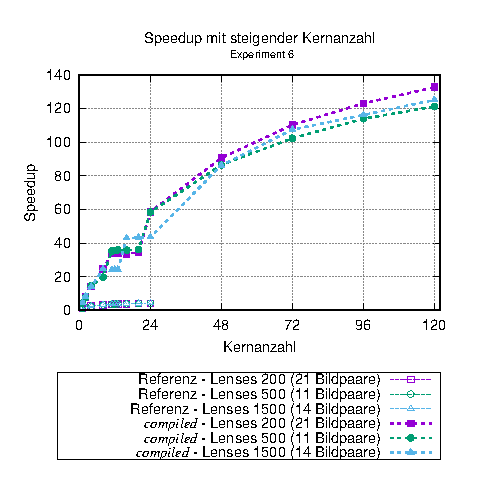
\includegraphics[width=\textwidth]{pdf/best_speedup_exp6}
		\caption{xperiment 6}
		\label{fig:best_speedup_exp6}
	\end{subfigure}
	\hfill
	\begin{subfigure}[b]{0.45\textwidth}
		\centering
		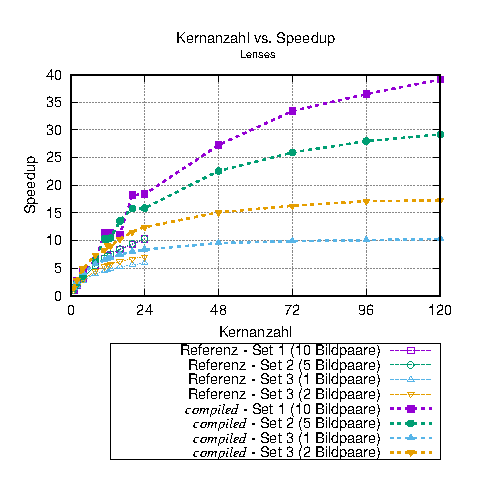
\includegraphics[width=\textwidth]{pdf/best_speedup_lenses}
		\caption{Lenses}
		\label{fig:best_speedup_lenses}
	\end{subfigure}
	\caption{Speedup der \textit{compiled} Implementierung gegenüber des vorgegebenen Python-Codes}
	\label{fig:best_speedup}
\end{figure}
\end{center}

Trotz dessen, dass mit 120 \gls{CPU}-Kernen bereits ein Speedup von über 130 erreicht wurde, müsste die Anzahl der Bildpaare und der Kerne bei weitem höher sein, um eine Echtzeitlauf des Programmes sicher zu stellen. Dies ist in Größenordnungen von 2400 Bildpaaren und 2400 \gls{CPU}-Kernen zu erwarten, was bereits 100 Taurus-Knoten sind. 

\begin{correctmore}
	- Analyse des erreichten Ergebnisses mit Rückblick auf die Möglichkeiten
	- Analyse des noch nicht genutzten Potentials mit Rückblick auf die Möglichkeiten
\end{correctmore}

\section{Verbesserungsmöglichkeiten}

Trotz dessen, dass in dieser Arbeit bereits viele Optimierungen implementiert wurden und ein hoher Speedup erreicht wurde, gibt es immer noch weiteres Potential. Die Verwendung der FFTW\footnote{\url{http://www.fftw.org/}} Bibliothek ist eine davon. Mithilfe dieser ist es möglich, die Gradientenintegration zu beschleunigen indem beim Start des Programmes sogenannte \textit{Wisdoms} erstellt werden, welche die Transformation eines Bildes in den Frequenzraum erheblich beschleunigen könnte. 

Des Weiteren ist es möglich für die meist aufgerufenen Funktionen Datenblöcke zu bilden und diese zu verarbeiten, sodass der Overhead für den Funktionsaufruf sinkt. Dies bildet ebenfalls eine gute Grundlage um diese Datenblockverarbeitung mittels numpy, numexpr oder numba weiter zu beschleunigen. Insbesondere kann hierbei auch die CUDA und OpenCL Schnittstelle von numba genutzt werden, um Berechnungen auf \glspl{GPGPU} auszulagern. 

Eine weitere Verbesserungsmöglichkeit liegt in einer Verbesserung des Belastungsausgleiches. Hierbei bestünde die Möglichkeit die Bildpaare in Packete zusammenzufassen und diese hintereinander auszuführen, sodass ein durchgängiger Betrieb möglich wäre. 

Auch Optimierungen am Algorithmus sind noch denkbar. Da aus dem Ergebnis des Template-Matchings nur die Position und der Wert des Maximums benötigt werden, ließe sich Bild und Template mit durch Skalierung verminderter Auflösung matchen. Hierbei entstandene Ungenauigkeiten können behoben werden, indem in der Region des Maximums ein genaueres Match durchgeführt wird. Da das Match mit reduzierter Auflösung eine Heuristik über die Maximal mögliche Übereinstimmung ist, kann anschließend in diesem der zweit höchste Wert betrachtet werden. Ist dieser größer als das Ergebnis des genauen Matches, besteht die Möglichkeit, dass dieses falsch ist und es kann auf den in der OpenCV-Bibliothek implementierten Template-Matching-Algorithmus zurückgreifen. Ist die Auflösung des Templates und des Bildes jedoch nicht durch ein und denselben Skalierungsfaktor teilbar, so kann die Skalierung auf eine niedrigere Auflösung bereits erhebliche Zeit in Anspruch nehmen. 

Zu guter Letzt besteht auch noch die Möglichkeit der Optimierung des Kalibrierungsteiles des Programmes. 